\chapter{Results of the cross-section measurement}
\minitoc

In this chapter results of the W/Z cross-section measurements will be discussed. 
In Sec. \ref{sec:flavCs} the cross-sections measured in each lepton flavors are presented. These results are used to test lepton universality in 2.76 TeV data.

Section \ref{sec:CombCs} describes a results obtained for combined W and Z cross-sections. Additionally, the cross-section ratios are presented. In Sec. \ref{sec:CompCs} the combined cross-sections are compared to the theoretical NLO predictions for different PDF sets. Finally, the results of cross-section measurement are interpreted using PDF profiling.

\section{Cross-sections results}\label{sec:flavCs}

The cross-sections are calculated as described in Chap.~\ref{chap:Met}. Table \ref{tab:Values} reports the number of candidates, the estimated background events and $C_{W/Z}$, $A_{W/Z}$ and $E_{W/Z}$ used in a different measurements are presented. 

The total uncertainty of the measurements in the fiducial region consists of the statistical, systematical and luminosity errors. The methods of these uncertainties determination are described in Chap. \ref{chap:Unc}. Uncertainty coming from luminosity measurments is labeled lumi. and is considered to be correlated for each channel. The statistical uncertainty is labeled stat. and is a dominant one for Z measurements and W boson measurements in electron channel. For W boson in electron channel the systematic uncertainty is around 1\%, that makes it significantly lower, than a statistical uncertainty. For W boson in a muon channel cross-sections the overall systematical uncertainty is higher because of the trigger scale factors, and is around 1.2\%, that makes it comparable with the statistical uncertainty. 

%\begin{table}[!tbp]
\begin{center}
\caption{Number of observed candidates N and expected background events B, efficiency, acceptance and extrapolation correction factors for the W and Z bosons in electron and muon channels. Monte Carlo corrections are included in the $C_{W/Z}$ factors. The given uncertainties are the quadratic sum of statistical and systematic components.}
\label{tab:Values}
\begin{tabular}{l | c c c c }
\hline
\hline
 & $N_{W/Z}^{sig}$ & $C_{W/Z}$ & $A_{W/Z}$ & $E_{W/Z}$ \\
 \hline
& \multicolumn{4}{c}{Electron channel}\\
 \hline
 $W^{+}\to e\nu$  & & & & \\
 $W^{-}\to e\nu$ & & & & \\
 $Z \to ee$ & & & & \\
 \hline
 & \multicolumn{4}{c}{Muon channel} \\
  \hline
  $W^{+}\to \mu\nu$  & & & & \\
 $W^{-}\to \mu\nu$ & & & & \\
 $Z \to \mu \mu $ & & & & \\
 \hline
\end{tabular}
\end{center}
\end{table}

\begin{table}[!tb]
\caption{Results on a fiducial $\sigma^{fid}$ and total cross-section measurement for $W^{+}$, $W^{-}$ and Z bosons in electron and muon channels. The cross-sections are shown with their statistical, systematical and luminosity uncertainties (and extrapolation error for total cross-section) quoted in that order}
\label{tab:Wcs}
\begin{center}
\begin{tabular}{| l | c | c |}
\hline
 & value $\pm$ stat $\pm$ syst $\pm$ lumi ($\pm$ ext)& value $\pm$ stat $\pm$ syst $\pm$ lumi ($\pm$ ext) \\
 \hline
 \hline
 & \multicolumn{2}{c|}{W in electron channel}\\
& $W^{+}\to e\nu$ & $W^{-}\to e\nu$ \\

\hline
$\sigma^{fid}_{W}$ [pb]  & \sigfidWplusenunolabel & \sigfidWminenunolabel \\
$\sigma^{tot}_{W}$ [pb] & \sigtotWplusenunolabel & \sigtotWminenunolabel \\
$\sigma^{13}_{W}$ [pb] & \sigTrWplusenunolabel & \sigTrWminenunolabel \\
\hline
\hline
 & \multicolumn{2}{c|}{W in muon channel}\\
& $W^{+}\to \mu\nu$ & $W^{-}\to \mu\nu$\\
\hline
$\sigma^{fid}_{W}$ [pb] & \sigfidWplusmununolabel & \sigfidWminmununolabel \\
$\sigma^{tot}_{W}$ [pb]  & \sigtotWplusmununolabel & \sigtotWminmununolabel \\
$\sigma^{13}_{W}$ [pb]  & \sigTrWplusmununolabel & \sigTrWminmununolabel \\
\hline
%\hline
 %& \multicolumn{2}{c|}{$W^{+-}$ } \\
%& $W \to e\nu$ & $W \to \mu \nu$ \\
%\hline
%$\sigma^{fid}_{W}$ &  & \\
%$\sigma^{tot}_{W}$ & & \\
%$\sigma^{13}_{W}$ & & \\
%\hline
\hline
 & \multicolumn{2}{c|}{Z} \\
& $Z \to ee$ & $ Z \to \mu\mu$ \\
\hline
$\sigma^{fid}_{Z}$  [pb] &\sigfidZeenolabel &  \sigfidZmumunolabel \\
$\sigma^{tot}_{Z}$  [pb] & \sigtotZeenolabel & \sigtotZmumunolabel \\
$\sigma^{13}_{Z}$ [pb]  & \sigTrZeenolabel & \sigTrZmumunolabel \\
\hline
\end{tabular}
\end{center}
\end{table}

\subsection{Lepton universality test}

\begin{figure}[!tb]
\begin{center}
\begin{minipage}[h]{0.8\linewidth}
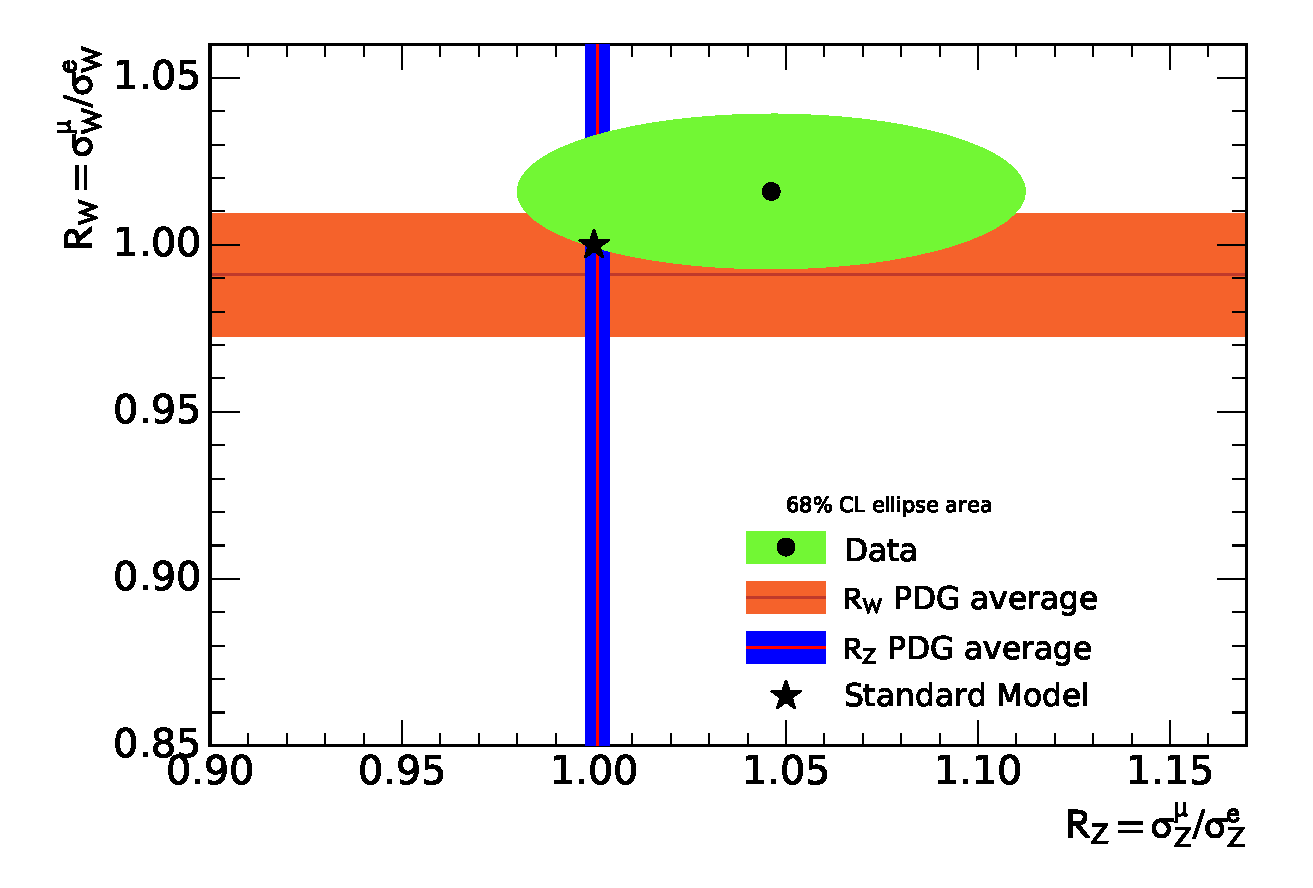
\includegraphics[width=1\textwidth]{Results/Univers.pdf}
\end{minipage}
\caption{The correlated measurement of the electron-to-muon fiducial cross-section ratios in the W and the Z channels. The vertical (horizontal) band represents the uncertainty of the cor- responding Z (W) branching fractions based on the current world average data. The green ellipse illustrates the 68\% CL for the correlated measurement of $R_W$ and $R_Z$.}
\label{fig:LeptUnivers}
\end{center}
\end{figure}


Because of the lepton universality of the Standard Model, the results, obtained in electron and muon channel are expected to agree with each other. The 2.76 TeV data could be used to test it via fiducial cross-section ratios of e and $\mu$ branching fractions:
\begin{center}
$R_{W}=\frac{\sigma^{\mu}_W}{\sigma^{e}_W} = \frac{BR(\wmunu)}{BR(\wenu)}= \valWunivers \pm \sysWunivers (sys.) \pm \statWunivers (stat.)$,
\end{center}
where the W cross-sections are calculated in fiducial region following the prescription from Sec. \ref{sec:Wcs}:
\begin{center}
$\sigma^{fid}_{W}(\wenu) = \valWenu  \pm \statWenu (stat.) \pm \sysWenu (sys.) \pm \lumiWenu (lumi.) \, [pb]$\\
$\sigma^{fid}_{W}(\wmunu) = \valWmunu  \pm \statWmunu (stat.) \pm \sysWmunu (sys.) \pm \lumiWmunu (lumi.) \, [pb]$
\end{center}
This result agrees within the uncertainty with the world average of $0.991\pm0.018$ \cite{Agashe:2014kda}. 

Similarly, this ratio can be measured in a Z boson decays as:
\begin{center}
$R_{Z}=\frac{\sigma^{\mu}_Z}{\sigma^{e}_Z} = \frac{BR(Z\to \mu\mu)}{BR(Z \to ee)}= \valZunivers \pm \sysZunivers(sys.) \pm \statZunivers (stat.)$
\end{center}
This ratio value is statistics dominated. The world average for a corresponding value is a $1.0009 \pm 0.0028$ \cite{Agashe:2014kda}. Comparison of the $R_W$ and $R_Z$ with the respect of the correlated systematic uncertainties with the world average is shown in Fig. \ref{fig:LeptUnivers}. The obtained values are agreeing withing the systematic uncertainty with the standard model expectations.




\section{Combined results}\label{sec:CombCs}

Since the results between channels are agreeing well, it is possible to perform averaging as described in Sec. \ref{sec:Aver}. The combination is done separately for fiducial, full and new 13 TeV cross-sections. Systematic uncertainties for the averaging are taken from Tab. \ref{tab:Unc}. The systematic uncertainties calculated using Toy MC are included in the averaging following the prescription from Sec. \ref{sec:Cor}. The common luminosity uncertainty is excluded from the combination process. The systematic uncertainties from electroweak background sources are considered uncorrelated between W and Z bosons and 100\% correlated for different W and Z channels.

The resulting cross-sections are summarized in Tab. \ref{tab:csComb}. The total systematic uncertainty for W cross-sections is below 2\%, what is smaller, than a statistical one, while the Z boson cross-sections uncertanties are fully dominated by the statistics. The uncertainties due to the extrapolation to the new 13 TeV common phase-space are also negligible. The luminosity uncertainty 3\% is fully correlated between the measurments.


The combination yields a good $\chi^2/NDF$=1.0/3 indicating good agreement between measurements. The combined cross-section is extrapolated to the full fiducial phase-space using $A_{W/Z}$ factors. 
\begin{table}[!tb]
\caption{Results on a fiducial $\sigma^{fid}$ and total cross-section measurement for $W^{+}$, $W^{-}$ and Z bosons in electron and muon channels. The cross-sections are shown with their statistical, systematical and luminosity uncertainties (and extrapolation error for total cross-section) quoted in that order}
\label{tab:csComb}
\begin{center}
\begin{tabular}{| l | c | c |}
\hline
 & value $\pm$ stat $\pm$ syst $\pm$ lumi ($\pm$ ext)& value $\pm$ stat $\pm$ syst $\pm$ lumi ($\pm$ ext) \\
 \hline
 \hline
 & \multicolumn{2}{c|}{$W^{+/-}$}\\
& $W^{+}\to l\nu$ & $W^{-}\to l\nu$ \\

\hline
$\sigma^{fid}_{W}$ [pb]  & $\valfidWp \pm \statfidWp \pm \sysfidWp \pm \lumifidWp$ & $\valfidWm \pm \statfidWm \pm \sysfidWm \pm \lumifidWm$ \\
$\sigma^{tot}_{W}$ [pb] & $\valfullWp \pm \statfullWp \pm \sysfullWp \pm \lumifullWp \pm \extrfullWp$ & $\valfullWm \pm \statfullWm \pm \sysfullWm \pm \lumifullWm \pm \extrfullWm$ \\
$\sigma^{13}_{W}$ [pb] & $\valthrWp \pm \statthrWp \pm \systhrWp \pm \lumithrWp$ & $\valthrWm \pm \statthrWm \pm \systhrWm \pm \lumithrWm$ \\
\hline
\hline
& \multicolumn{2}{c|}{$W \to l \nu$} \\
\hline
$\sigma^{fid}_{W}$ [pb] & \multicolumn{2}{c|}{$\valfidWtot \pm \statfidWtot \pm \sysfidWtot \pm \lumifidWtot$} \\
$\sigma^{tot}_{W}$ [pb]  & \multicolumn{2}{c|}{$\valfullWtot \pm \statfullWtot \pm \sysfullWtot \pm \lumifullWtot \pm \extrfullWtot$} \\
$\sigma^{13}_{W}$ [pb]  & \multicolumn{2}{c|}{$\valthrWtot \pm \statthrWtot \pm \systhrWtot \pm \lumithrWtot$} \\
\hline
%\hline
 %& \multicolumn{2}{c|}{$W^{+-}$ } \\
%& $W \to e\nu$ & $W \to \mu \nu$ \\
%\hline
%$\sigma^{fid}_{W}$ &  & \\
%$\sigma^{tot}_{W}$ & & \\
%$\sigma^{13}_{W}$ & & \\
%\hline
\hline
 & \multicolumn{2}{c|}{$Z \to ll$} \\
\hline
$\sigma^{fid}_{Z}$ [pb] & \multicolumn{2}{c|}{$\valfidZ \pm \statfidZ \pm \sysfidZ \pm \lumifidZ$} \\
$\sigma^{tot}_{Z}$ [pb]  & \multicolumn{2}{c|}{$\valfullZ \pm \statfullZ \pm \sysfullZ \pm \lumifullZ \pm \extrfullZ$} \\
$\sigma^{13}_{Z}$ [pb]  & \multicolumn{2}{c|}{$\valthrZ \pm \statthrZ \pm \systhrZ \pm \lumithrZ$} \\
\hline
\end{tabular}
\end{center}
\end{table}

\subsection{Cross-sections ratios}

Measurement of the ratios is a powerful tool to test PDF predictions, since it allows to cancell the biggest uncertainty coming from luminosity. The ratios for W/Z cross section have been calculated in a fiducial region following the prescription from Sec.~\ref{sec:Rat}. The obtained results are:

\begin{center}
$R_{W/Z} = \valfidWZ \pm \statfidWZ \, (stat.)\, \pm \sysfidWZ\, (sys.)\,  $ \\
$R_{W^{+}/Z} = \valfidWpZ \pm \statfidWpZ\, (stat.)\, \pm \sysfidWpZ \, (sys.)\, $ \\
$R_{W^{-}/Z} = \valfidWmZ \pm \statfidWmZ\, (stat.)\,  \pm \sysfidWmZ\,  (sys.)\, $ \\
$R_{W^{+}/W^{-}} = \valfidWpWm \pm \statfidWpWm\, (stat.)\, \pm \sysfidWpWm\,  (sys.)\,  $ \\
\end{center}


\section{Comparation with theoretical predictions}\label{sec:CompCs}

The theoretical predictions are calculated at NLO using MCFM\cite{MCFM} for a different PDF sets: ABM12nlo\cite{ABM12}, CT14nlo\cite{CT14}, MMHTnlo\cite{MMHT}, ATLAS-epWZnlo, HERAPDF2.0nlo in fiducial region. The MCFM is a parton-level Monte-Carlo generator, that gives a predictions at LO and NLO level. It is interfaces with APPLGRID\cite{APPLGRID}, that provides a $x$ vs $Q^2$ grid for MCFM. The comparison of cross-sections for a combined channes is shown in Fig. \ref{}. The theoretical predictions are agreeing with experimental results within 2$\sigma$, however, the difference for the ratios (Fig.\ref{}) is higher. 



\section{Effect on PDF distributions}\label{sec:PDFCs}

The effect of these cross-sections measurements estimated using PDF profiling method on CT10 nlo set with uncertainties estimated following prescription in Sec. \ref{sec:PDFFit}. The fit gives \chiD/NDF= , that showes a good agrement with data.  The impact is shown in Fig. \ref{}, where results, obtained using CT10 PDF set are compared to the profiled results with this measurement included. The impact of data on experimental uncertainties is not visible for most of the distribtions, however it slightly improves knowledge of valence quarks densities.